\section{Introduction}\label{sec:intro}

%% Motivation
% What's the big picture problem?
Fully Homomorphic Encryption (FHE) refers to any encryption scheme that allows for homomorphically adding and multiplying ciphertexts, so that the sum of the encryptions of two integers is an encryption of their sum, and similarly the product of the encryptions of two integers is an encryption of their product \cite{Gentry}.
While FHE is a powerful technique for carrying out privacy-preserving computations on encrypted data, it has a major downside: it is slow.
Homomorphic computations over ciphertexts are often orders of magnitude slower than a corresponding plaintext computation.
%\raghav{I wonder if reviewers will read this and think ``hmm there was a PLDI paper last year that said the same thing''}
Many FHE cryptosystems support packing large numbers of ciphertexts into {\em ciphertext vectors}, essentially compensating for the inherent slowness of FHE by enabling SIMD-style computation \cite{BrakerskiPacking,SmartPacking}.
To properly take advantage of ciphertext packing, we need a compiler that can vectorize arbitrary FHE programs.
% \raghav{It feels like I should mention ``all FHE programs are arithmetic circuits'' here, but I'm not sure where. One idea is it can go as part of the ``you can't do normal vectorization'' bit, since there are no loops and stuff to take advantage of. But I'm not sure.}\milind{I think what you've written here seems good.}

% Who has tried to solve this problem before?
Vectorizing compilers for FHE, such as CHET~\cite{CHET} and Porcupine~\cite{Porcupine}, exist.
However, neither of these approaches meets the need for a vectorizing compiler for arbitrary FHE programs.
While CHET is optimized for highly regular computations over packed tensors (such as neural networks), it does not generalize to more irregular programs. 
Porcupine, which uses a synthesis-based approach to generate vectorized code for arbitrary kernels, does work for a more general class of programs.
However, it is not automated, as it requires a programmer-provided {\em sketch} as a starting point.
%\raghav{Is there a better/more correct/more effective way to say this?}\milind{It also relies on loops as its source of vectorization, right? Or am I misemembering?}

% However, these prior approaches are optimized for highly regular computations over packed tensors (such as neural networks in the case of CHET), and often don't take into account how expensive rotations can be in more irregular applications.
% \milind{You might want to be a little more explicit about the comparisons here: CHET does X, which means it doesn't do Y. Porcupine does A, which means it has drawback B.}
% A lot of FHE computations do not deal with regular data structures like tensors, which makes it much harder to take advantage of vectorization opportunities.

Other approaches to vectorizing arbitrary, non-loop-based code, such as Superword-Level Parallelism~\cite{SLP}, also fail here.
SLP aggressively packs isomorphic instructions into vectors, because it assumes that shuffling vector lanes around or indexing into a vector is relatively cheap.
In FHE, however, the vectors are not physical vector registers with slots for data: %, but rather {\em abstract mathematical objects} which only {\em encode} several ciphertexts.
the only way to move data between vector lanes in FHE is by performing a cyclic rotation of the entire vector.
Realizing the shuffles incurred by SLP with a series of masks and rotates is expensive, and can quickly outweigh any benefits from vectorizing.
% While it is theoretically possible to encode arbitrary permutations as a series of masks and rotates, realizing the shuffles incurred by SLP in this way can quickly outweigh any benefits from vectorizing in the first place. 

%\raghav{Still need to review this for accuracy}
More recent takes on SLP, such as VeGen \cite{VeGen} and goSLP \cite{goSLP}, recognize the need to take the cost of data movement into account.
VeGen 
%incorporates data movement into its vectorization, and 
can decide to not pack certain instructions together because the data movement cost incurred is not worth it.
However, VeGen does its reasoning {\em locally}; that is, it cannot reason about the effect packing instructions together may have on shuffling costs much later in the program. This tradeoff, fine in circumstances when shuffling is relatively cheap, is inappropriate for FHE, where shuffling is very expensive.
While goSLP does reason globally, the cost model it uses to avoid over-packing is incompatible with the semantics of FHE vectorization.
We discuss this further in Section~\ref{sec:related-work}.

\subsection*{The vectorization/rotation tradeoff}

In general, without carefully accounting for, and controlling, rotation, traditional vectorization strategies can lead to {\em slowdowns}, rather than speedup, in an FHE setting. It is often beneficial to give up vectorization opportunities to avoid incurring expensive rotations.

\begin{figure}
    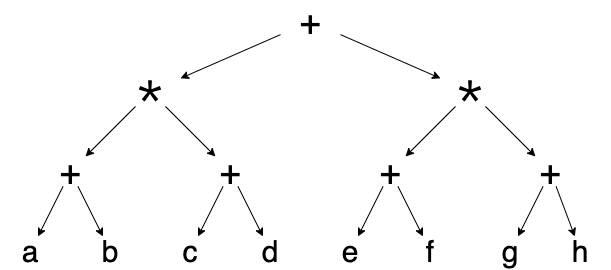
\includegraphics[width=0.9\linewidth]{figures/compilation_overview/coyote_running_example.drawio.png}
    % \vspace{-1em}
    \caption{An example of an arithmetic circuit}\label{fig:example-circuit}
    \Description{A figure of an arithmetic circuit computing ((a + b) * (c + d)) + ((e + f) * (g + h))}
\end{figure}


\begin{figure}
\small
    \begin{subfigure}{0.4\columnwidth}
%         \begin{verbatim}
% %0 = a + b
% %1 = c + d
% %2 = %0 * %1
% %3 = e + f
% %4 = g + h
% %5 = %3 * %4
% %6 = %2 + %5
%         \end{verbatim}
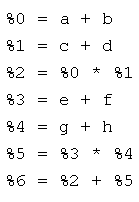
\includegraphics[width=0.6\linewidth]{figures/possible_schedules/no_vectorization.drawio.pdf}
        % \vspace{-1em}
        \caption{No vectorization}\label{fig:no-vectorization}
    \end{subfigure}
    \begin{subfigure}{0.6\columnwidth}
%         \begin{verbatim}
% [%0, %1, %3, %4] = [a, c, e, g] + 
%                     [b, d, f, h]
% [%2, _, %5, _] = [%0, _, %3, _] * 
%                     [%1, _, %4, _]
% [%6, _, _, _] = [%2, _, _, _] + 
%                     [%5, _, _, _]
%         \end{verbatim}
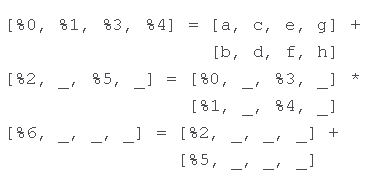
\includegraphics[width=0.9\linewidth]{figures/possible_schedules/aggressive_vectorization.drawio.pdf}
        \vspace{-1em}        
        \caption{Aggressive vectorization, incurs two rotates}\label{fig:aggressive-vectorization}
    \end{subfigure}
    \begin{subfigure}{0.8\columnwidth}
        \centering
        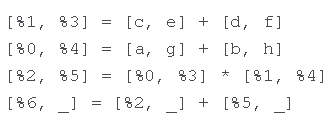
\includegraphics[width=0.7\linewidth]{figures/possible_schedules/optimal_schedule.drawio.pdf}
%         \begin{verbatim}
% [%1, %3] = [c, e] + [d, f]
% [%0, %4] = [a, g] + [b, h]
% [%2, %5] = [%0, %3] * [%1, %4]
% [%6, _] = [%2, _] + [%5, _]
%         \end{verbatim}
        \vspace{-1em}        
        \caption{Optimal schedule, incurs one rotate}\label{fig:optimal-schedule}
    \end{subfigure}
    % \vspace{-1em}
    \caption{Possible schedules for Figure~\ref{fig:example-circuit}}
    \Description{Three possible schedules for an arithmetic circuit; one is scalar, one is aggressively vectorized, and one trades off between the two extremes.}
\end{figure}

%\raghav{TODO: find a better place to put this paragraph, maybe?}
%
Consider the arithmetic circuit in Figure~\ref{fig:example-circuit} implementing $((a + b) * (c + d)) + ((e + f) * (g + h))$.\footnote{We adopt the FHE-standard representation of arithmetic circuits as the intermediate representation for our programs~\cite{Gentry,CircuitRewriting,Ramparts,Porcupine}.}
A na\"ive vectorization would pack together the four additions at the first level, and the two multiplies at the second level (as in the schedule in Figure~\ref{fig:aggressive-vectorization}).
The resulting schedule has a vector add, followed by a vector multiply, followed by an add. Rotations are needed between each operation to align the outputs of each operation with the next.
Using an approximate model\footnote{\citet{AlgosHElib} assigns a ``high latency'' to both multiplies and rotates and a ``low latency'' to adds. For both simplicity and concreteness, we assume a 10:1 ratio between ``high latency'' and ``low latency.''} of the relative latencies of each instruction in which multiplies and rotates have a latency of 1 and addition has a latency of 0.1, the total cost of this schedule is 3.2.
However, by doing no vectorization and executing the circuit entirely with scalar operations (Figure~\ref{fig:no-vectorization}), we have five adds and two multiplies, with an overall cost of 2.5.
In this case, vectorization actually makes the performance {\em worse}!
Figure~\ref{fig:optimal-schedule} shows how we can do better:
We pack the $a+b$ and the $e+f$ adds separately from the $c+d$ and $g+h$ adds, so that neither of them require a rotation to align with the multiply above them.
By saving one rotation at the cost of an extra vector addition, we get a schedule with an overall cost of only 2.3.
% \raghav{further TODO: dunno how much detail I should be going into here. Should I enumerate the nodes of the circuit and refer to them explicitly? Or insert a sample of the vectorized code in both cases? Or something else? As it is, I'm certain this is pretty hard to follow.}
% \milind{I tried to make this simpler, but it might be good to shrink the tree in Figure 1, and put three subfigures next to it showing the three schedules.}\raghav{Schedules like the ones in Figure~\ref{fig:aligned-schedule}?}\milind{yes.}

We need a new arbitrary vectorization strategy that is {\em FHE-aware}; i.e., it packs instructions without relying on regularity in the original computation, and can still account for the high cost of data movement throughout the program.

\subsection*{Co-optimization of vector packing and data layout}
%\milind{check}\raghav{I like it}
Our key insight is that because rotations are so expensive, data layout and vector packing are fundamentally intertwined. Rather than treat these as separate problems, we must optimize them {\em together} when finding a schedule.
The main obstacle to optimality when using the classical approach is simple: vectorizing across instructions by aggressively packing them into vectors can require substantial, and complex, data movement to align operands for downstream vector instructions (e.g., SwizzleInventor \cite{SwizzleInventor}, which resorts to sketch-based synthesis to generate the appropriate permutations). If permuting operands between lanes can only be done with expensive rotations, an aggressively packed schedule can incur so much overhead that no amount of vectorization makes it worth it.

Instead, we develop an approach that works at the level of {\em subcircuits}, splitting the program up into smaller pieces within which all the computations are locked into a single lane to avoid doing any rotations at all. While vectorizing across subcircuits gives up some packing potential (because operations within a subcircuit cannot be vectorized together), the savings on rotation costs can make up the difference: the subcircuits prevent over-vectorization that incurs too many rotations. The optimal schedule of Figure~\ref{fig:optimal-schedule} can be viewed as grouping $(a + b)$ with its downstream multiply in one subciruit, and $(g + h)$ with its downstream multiply in another subcircuit, and then vectorizing those two subcircuits together.

This approach yields a natural question: how do we decide which computations to merge into a subcircuit? This seems circular: subcircuit merging is intended to yield fewer rotations, which are determined by data layout, and data layout is driven by which operations are vectorized together, which in turn is constrained by subcircuit identification. 


\subsection*{Contributions}

This paper presents \system, the first vectorizing, FHE-aware compiler for programs that do not have regular structure. \system breaks the circular dependence between vector packing and data layout by using an iterative process that alternates between making packing decisions and determining data layout. \system uses simulated annealing to find optimal data layouts, and uses these to guide a best-first search towards optimal vector packs. Crucially, \system uses layouts from previous iterations of scheduling to identify profitable subcircuits to merge, and then re-schedules based on the new subcircuits.


Rather than incurring many expensive data shuffles by aggressively vectorizing the whole program, \system's subcircuit-based scheduling and FHE-specific cost model co-optimize the data layout and vector packing, producing a schedule that enjoys the benefits of vectorization while still being able to efficiently realize the necessary rotations. For example, \system is able to correctly generate the better vectorization schedule in Figure~\ref{fig:optimal-schedule}.

%\milind{High level idea of find subcircuits -> vectorize subcircuits -> do layout -> tweak subcircuits}\raghav{Is this the right level of generality?}

% \raghav{feels weird explicitly saying irregular here, should I say `arbitrary' instead?}\milind{How's that?}\raghav{Good, I think. I just don't want to seem like we're claiming that Coyote is {\em specifically for irregular things} and then be left with a disconnect between that claim and the fact that many of our benchmarks are, ostensibly, pretty regular.}


%\milind{two sentences or so about simulated annealing...}\raghav{Is this accurate? Does it make sense? Right level of generality?}

The specific contributions we make are:
\begin{enumerate}
    \item An algorithm for simultaneously searching the space of data layouts and the space of vector packings to find an efficient combination. %automatically identifying vectorizable structures in a program
    % \item An algorithm for optimally choosing data layout to minimize the total cost of moving data around
    \item A lightweight Python embedded DSL called \system, with a compiler that uses this algorithm to generate efficient FHE code for arbitrary programs
\end{enumerate}

%% Results
We tested \system by using it to compile five computational kernels (matrix multiply, point cloud distances, 1D convolution, dot product, and decision tree traversal), and compared the performance of the vectorized code to to the original unvectorized code.
We also randomly generated several irregular polynomial-evaluation programs to measure the effect of things like operation density on \system's ability to vectorize. 
We find that \system very effectively vectorizes programs, yielding efficient vector schedules with optimized rotations.

%The remainder of this paper is organized as follows. Section~\ref{sec:background} gives background on FHE and vectorization. Section~\ref{sec:overview} overviews \system. Section~\ref{sec:design} dives into the key components of \system's design: selecting which operations to vectorize together, and how to assign those operations to lanes. Section~\ref{sec:implementation} describes the implementation, including tradeoffs between speed and optimality that \system makes. Section~\ref{sec:eval} evaluates \system. Section~\ref{sec:related-work} discusses related work, and Section~\ref{sec:conclusion} concludes.
